\section{Introduction}

Deploying a physiological monitoring model across hospitals begins with a step no model
can skip: deciding which channel is which. \texttt{itemid 220045} in one intensive-care
database and \texttt{Vital Signs|Heart Rate} in another carry the same signal; a third
field named \texttt{Heart Rate} in a nurse-charting table does not. Of the $135$ concepts
we align, $63$ are continuously monitored channels, and eICU's periodic vitals table
alone holds $5.5\times10^{8}$ samples of them. A mis-assigned channel is a signal-level
defect: a temperature series concatenated across Celsius and Fahrenheit sources, or an
arterial line merged with a cuff, corrupts every filter computed downstream.

Existing approaches to this alignment fall into two families. \emph{Curated dictionaries}
map each database by hand into a shared concept
vocabulary~\cite{ricu,ohdsi,mimiccode}. They are accurate but partial by construction:
\texttt{ricu} maps $119$ concepts across five databases and states that its dictionary is
not comprehensive, and the three public expert mappings we use agree with one another at
pairwise Jaccard $0.29$--$0.42$. \emph{Automatic schema
matching} instead learns or prompts the correspondence~\cite{rahm2001,llmatch,bdiviz}.
Both families share an assumption that the clinical setting violates: that every source
attribute has a target. They also assume the metadata a matcher would use is present,
whereas four eICU tables covering $319$ fields and $7.3\times10^{8}$ rows carry no unit
column at all.

Given this, one expects automatic alignment to be hard. It is not---at least not the part
usually measured. A frozen language model prompted with the schema-matching template of
LLMatch~\cite{llmatch}, shown only dictionary labels and training-split aggregates, ranks
the correct concept first for $95.9$, $97.3$ and $88.2\%$ of mappable fields on MIMIC-IV,
MIMIC-III (CareVue) and eICU. The difficulty lies in the complement: of the fields
recorded for at least $5\%$ of stays, $77.1\%$ belong to no concept in our $138$-concept
catalogue---site-local assays, device settings, free-text flags, nursing observations.
Precision is consequently only $69$--$85\%$, and an error decomposition attributes
$90.5\%$ and $93.0\%$ of errors on MIMIC-IV and CareVue to assigning a concept to a field
that has none. The binding problem is abstention, not ranking.

Abstention is well studied as selective prediction and open-set
recognition~\cite{selective,openset,msp}, but there the thresholded confidence comes from
the classifier's own output distribution. A generative matcher has no such distribution:
it emits an accept/reject decision with no graded score. A natural substitute is to
reject implausible matches with deterministic compatibility rules---a field in
\textsc{mg/dL} cannot realise a concept in \textsc{mmHg}; a field assayed on ascites
cannot realise a serum concept. Used that way the rules \emph{lose}, costing
$2.6$--$10.2$ Recall@1 points for no consistent detection gain, because the matcher
already respects them in $99.3$--$100\%$ of accepted matches. Motivated by this
observation, we move the same signal to a different position in the pipeline: rather than
deciding \emph{which} concept a field takes, the checks score how much evidence
contradicts the match already made, and that score becomes the abstention criterion.

Our main contributions are three folds: (1) We propose reading deterministic unit, data
type and specimen compatibility as \emph{abstention evidence} rather than as a
re-ranking filter, which improves open-set AUROC by $5.7$ points on two of three
databases without changing which concept is proposed, and we isolate the effect with a
controlled comparison that holds the penalty, its weight, the candidates and the
calibration split fixed and varies only what consumes the signal. (2) We release a
three-database field-level reference standard for open-set alignment---$710$
field--concept pairs covering $135$ of $138$ catalogue concepts, and $2{,}428$ adjudicated
\textsc{unknown} fields drawn from real schemas rather than constructed as
negatives---validated by two blinded independent human experts ($\kappa{=}0.952$).
(3) We show the effect replicates across three language-model families and quantify what
alignment quality is worth downstream, in a zero-shot cross-database transfer of a
$24$-channel physiological time-series model.

\begin{figure*}[t]
\centering
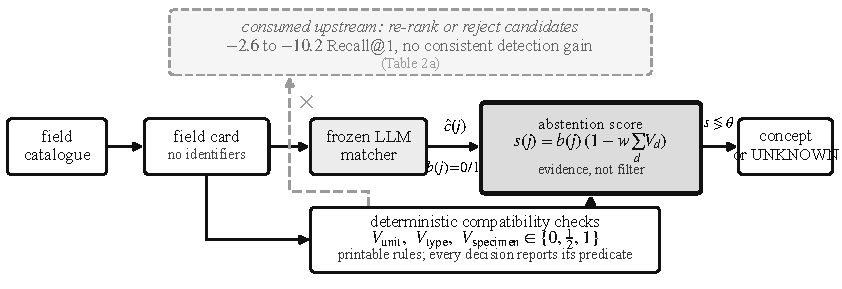
\includegraphics[width=0.88\textwidth]{figures/method.pdf}
\caption{The overall architecture of the proposed method. Deterministic compatibility
checks are read as evidence about a match the frozen matcher has already made: they
discount the confidence $b(j)$ attached to $\hat{c}(j)$ and never change which concept is
proposed. Consuming the identical penalty one step earlier---to re-rank or reject
candidates---costs $2.6$--$10.2$ Recall@1 points for no consistent detection gain
(Table~\ref{tab:ablate}a).}
\label{fig:arch}
\end{figure*}
